% \documentclass[aspectratio=169, xcolor=table]{beamer} % 16:9 Widescreen

% % ---------------------------------------------------
% % CUSTOM COLORS & TYPOGRAPHY (MATCH YOUR TEMPLATE)
% % ---------------------------------------------------
% % Change these RGB values to match your university/template colors
% \definecolor{PrimaryColor}{RGB}{12, 45, 89}   % Deep Corporate Blue
% \definecolor{SecondaryColor}{RGB}{0, 163, 224} % Lighter Accent Blue
% \definecolor{LightGrey}{RGB}{240, 242, 245}

% \usefonttheme{professionalfonts} % Cleaner math and text fonts
% \renewcommand{\familydefault}{\sfdefault} % Modern sans-serif default

% % ---------------------------------------------------
% % BEAMER STYLING OVERRIDES
% % ---------------------------------------------------
% \setbeamertemplate{navigation symbols}{} % Remove clunky navigation icons
% \setbeamertemplate{itemize items}[circle] % Clean circle bullets
% \setbeamercolor{structure}{fg=PrimaryColor} % Bullet colors
% \setbeamercolor{frametitle}{bg=PrimaryColor, fg=white} % Header bar
% \setbeamercolor{title}{bg=PrimaryColor, fg=white}
% \setbeamercolor{block title}{bg=SecondaryColor, fg=white}
% \setbeamercolor{block body}{bg=LightGrey, fg=black}

% % Custom Footer (Author, Title, Slide Number)
% \setbeamertemplate{footline}{
%   \leavevmode%
%   \hbox{%
%   \begin{beamercolorbox}[wd=.333333\paperwidth,ht=2.25ex,dp=1ex,center]{author in head/foot}%
%     \usebeamerfont{author in head/foot}\insertshortauthor
%   \end{beamercolorbox}%
%   \begin{beamercolorbox}[wd=.333333\paperwidth,ht=2.25ex,dp=1ex,center]{title in head/foot}%
%     \usebeamerfont{title in head/foot}\insertshorttitle
%   \end{beamercolorbox}%
%   \begin{beamercolorbox}[wd=.333333\paperwidth,ht=2.25ex,dp=1ex,right]{date in head/foot}%
%     \usebeamerfont{date in head/foot}\insertframenumber{} / \inserttotalframenumber\hspace*{2ex} 
%   \end{beamercolorbox}}%
%   \vskip0pt%
% }

% % Automated Section Transition Slides
% \AtBeginSection[]{
%   \begin{frame}
%   \vfill
%   \centering
%   \begin{beamercolorbox}[sep=8pt,center,shadow=false,rounded=true]{title}
%     \usebeamerfont{title}\insertsectionhead\par%
%   \end{beamercolorbox}
%   \vfill
%   \end{frame}
% }

% % ---------------------------------------------------
% % PRESENTATION METADATA
% % ---------------------------------------------------
% \title[SRP Architecture]{MLPs with Attention (V2) (SRP)}
% \subtitle{An End-to-End Neural Ensemble with Causal Transformer Blocks \\ \& Deep Supervision}
% \author[Team Name]{Your Name / Team Name}
% \institute[Uni Hildesheim]{
%     \textbf{University of Hildesheim} \\ 
%     \vspace{0.2cm}
%     \textit{Interim Presentation 2025} \\
%     \textit{Supervisor: [Insert Name]}
% }
% \date{\today}

% \begin{document}

% % --- TITLE SLIDE ---
% \begin{frame}[plain] % [plain] removes the footer for a cleaner cover
%     \titlepage
% \end{frame}

% % --- AGENDA ---
% \begin{frame}{Agenda}
%     \tableofcontents[hideallsubsections]
% \end{frame}

% % ---------------------------------------------------
% % SLIDES
% % ---------------------------------------------------

% \section{Introduction to SRP}

% \begin{frame}{Introduction \& Motivation}
%     \begin{columns}
%         \column{0.5\textwidth}
%         \textbf{The Concept:} 
%         \vspace{0.2cm}
%         \\
%         SRP is a neural architecture designed for tabular data that treats feature extraction as a sequential process of refinement.
%         \vspace{0.4cm}
%         \\
%         \textbf{Analogy to GBDT:}
%         \vspace{0.2cm}
%         \\
%         Much like Gradient Boosted Trees (XGBoost), SRP builds complexity step-by-step, but remains fully differentiable and end-to-end trainable in PyTorch.
        
%         \column{0.5\textwidth}
%         \begin{block}{The "Information Staircase"}
%             Instead of a single monolithic network, data is processed sequentially where later stages have full visibility of earlier feature extraction.
%         \end{block}
%     \end{columns}
% \end{frame}

% \section{Problem Formulation}

% \begin{frame}{Problem Formulation}
%     \begin{itemize}
%         \setlength\itemsep{1em}
%         \item \textbf{Input:} A feature vector $X \in \mathbb{R}^d$ (e.g., coordinates, income, age).
%         \item \textbf{Internal Sequence:} $X$ is projected into $K$ embeddings by $K$ independent ``Weak Learners.''
%         \item \textbf{Causal Constraint:} Each step $i$ can only attend to the outputs of steps $1 \dots i$.
%         \item \textbf{Output:} A sequence of $K$ predictions:
%         \begin{equation*}
%             \hat{y}_1, \hat{y}_2, \dots, \hat{y}_K
%         \end{equation*}
%         \item \textbf{Objective:} Maximize the predictive power of the final step $\hat{y}_K$ while utilizing previous steps as auxiliary tasks.
%     \end{itemize}
% \end{frame}

% \section{Architecture Overview}

% \begin{frame}{Architecture: Weak Learner Ensembles}
%     \begin{columns}
%         \column{0.55\textwidth}
%         \textbf{Design of Weak Learners:}
%         \begin{itemize}
%             \item Small, constrained MLPs (1-2 layers, 8-16 neurons).
%             \item \textbf{Constraint:} Keeping learners ``weak'' forces the Transformer to learn global interactions rather than relying on a single path.
%         \end{itemize}
        
%         \column{0.4\textwidth}
%         \begin{block}{Regularization}
%             L1/L2 penalties are applied to ensure feature sparsity and prevent early-sequence dominance.
%         \end{block}
%     \end{columns}
% \end{frame}

% \begin{frame}{Architecture: Causal Transformer Blocks}
%     \begin{itemize}
%         \setlength\itemsep{1em}
%         \item \textbf{Causal Masking:} A strict upper-triangular mask ensures the ``Information Staircase'' is maintained.
%         \item \textbf{Residual Connections:} Mathematically stabilizes the deep network:
%         \begin{equation*}
%             x_{out} = \text{LayerNorm}(x_{in} + \text{CausalAttention}(x_{in}))
%         \end{equation*}
%         \item \textbf{Non-linear Head:} A 2-layer MLP head with SiLU activation transforms the final 32D attention space into the target value.
%     \end{itemize}
% \end{frame}

% \section{Methodology}

% \begin{frame}{Methodology: Weighted Deep Supervision}
%     \begin{block}{Deep Supervision Objective}
%         Mean Squared Error (MSE) is calculated at \textit{every} step of the sequence.
%     \end{block}
%     \vspace{0.3cm}
%     \begin{itemize}
%         \item \textbf{The Weighting Problem:} Linear weighting $(w_i = i/K)$ punishes early learners for not knowing the ``whole story,'' destabilizing gradients.
%         \item \textbf{The Solution (Exponential Weighting):}
%         \begin{equation*}
%             w_i = \frac{2^i}{\sum_{j=1}^K 2^j}
%         \end{equation*}
%         \item \textbf{Result:} Early steps receive tiny weights (acting as regularizers). The final step receives maximum weight, focusing the optimizer on the most informed tokens.
%     \end{itemize}
% \end{frame}

% \section{Data Preprocessing}

% \begin{frame}{Preprocessing: Non-linear Transformations}
%     \begin{columns}
%         \column{0.5\textwidth}
%         \textbf{StandardScaler Limitation}
%         \vspace{0.2cm}
%         \\
%         Assumes a Gaussian distribution. It fails to stabilize gradients when dealing with heavy-tailed, non-linear tabular data (like housing prices).
        
%         \column{0.5\textwidth}
%         \textbf{QuantileTransformer}
%         \vspace{0.2cm}
%         \\
%         \begin{itemize}
%             \item Maps features to a strict Standard Normal distribution based on rank.
%             \item Collapses outliers aggressively.
%             \item \textbf{Impact:} Provides a strictly bounded input space, vastly improving SRP performance.
%         \end{itemize}
%     \end{columns}
% \end{frame}

% \section{Experimental Results}

% \begin{frame}{Experimental Setup}
%     \begin{table}
%         \centering
%         \renewcommand{\arraystretch}{1.3} % Adds padding to rows
%         \begin{tabular}{l | l}
%             \rowcolor{PrimaryColor} \color{white}\textbf{Parameter} & \color{white}\textbf{Configuration} \\
%             Dataset & California Housing (80/20 Split) \\
%             \rowcolor{LightGrey} Optimizer & AdamW ($lr=1e-3$) \\
%             Learners ($K$) & 24 \\
%             \rowcolor{LightGrey} Embedding Dim. & 32 \\
%             Attention Depth & 2 Blocks \\
%             \rowcolor{LightGrey} Activation & SiLU \\
%         \end{tabular}
%     \end{table}
% \end{frame}

% \begin{frame}{Results \& Key Findings}
%     \begin{itemize}
%         \setlength\itemsep{1em}
%         \item \textbf{Overall Performance:} Achieved a final validation $R^2$ of \textbf{$\sim$0.81}, bridging the gap between standard MLPs and tree-based ensembles.
%         \item \textbf{Impact of Weighting:} Exponential weighting improved gradient stability and final accuracy by 15\% compared to inverse or linear schemes.
%         \item \textbf{Ablation Insight:} Residual Connections and LayerNorm are absolute prerequisites for training the depth of the transformer block successfully.
%     \end{itemize}
% \end{frame}

% % --- Q&A SLIDE ---
% \begin{frame}[plain]
%     \vfill
%     \begin{center}
%         \textcolor{PrimaryColor}{\Huge \textbf{Thank You}} \\
%         \vspace{0.8cm}
%         \large \textbf{Questions \& Discussion} \\
%         \vspace{0.5cm}
%         \normalsize 
%         \textit{Email:} [Your Email] \\
%         \textit{GitHub:} [Your Repo Link]
%     \end{center}
%     \vfill
% \end{frame}

% \end{document}
%asdasdasdasd

% \documentclass[aspectratio=169, xcolor=table]{beamer} % 16:9 Widescreen

% % ---------------------------------------------------
% % CUSTOM COLORS & TYPOGRAPHY (MATCH YOUR TEMPLATE)
% % ---------------------------------------------------
% % Update these to your university's exact colors if known
% \definecolor{PrimaryColor}{RGB}{12, 45, 89}   % Deep Corporate Blue
% \definecolor{SecondaryColor}{RGB}{0, 163, 224} % Lighter Accent Blue
% \definecolor{LightGrey}{RGB}{240, 242, 245}

% \usefonttheme{professionalfonts} % Cleaner math and text fonts
% \renewcommand{\familydefault}{\sfdefault} % Modern sans-serif default

% % ---------------------------------------------------
% % BEAMER STYLING OVERRIDES
% % ---------------------------------------------------
% \setbeamertemplate{navigation symbols}{} % Remove clunky navigation icons
% \setbeamertemplate{itemize items}[circle] % Clean circle bullets
% \setbeamercolor{structure}{fg=PrimaryColor} % Bullet colors
% \setbeamercolor{frametitle}{bg=PrimaryColor, fg=white} % Header bar
% \setbeamercolor{title}{bg=PrimaryColor, fg=white}
% \setbeamercolor{block title}{bg=SecondaryColor, fg=white}
% \setbeamercolor{block body}{bg=LightGrey, fg=black}

% % ---------------------------------------------------
% % LOGO ON EVERY SLIDE
% % ---------------------------------------------------
% \usepackage{textpos}
% \addtobeamertemplate{frametitle}{}{%
% \begin{textblock*}{2cm}(12.8cm,-1.2cm) % Adjust these coordinates if the logo needs to move
% 
\includegraphics[height=1.8cm,width=3cm,keepaspectratio]{uni logo.png}
% \end{textblock*}}

% % ---------------------------------------------------
% % CUSTOM FOOTER (Title & Slide Number ONLY)
% % ---------------------------------------------------
% \setbeamertemplate{footline}{
%   \leavevmode%
%   \hbox{%
%   \begin{beamercolorbox}[wd=.5\paperwidth,ht=2.25ex,dp=1ex,left]{title in head/foot}%
%     \hspace*{2ex}\usebeamerfont{title in head/foot}\insertshorttitle
%   \end{beamercolorbox}%
%   \begin{beamercolorbox}[wd=.5\paperwidth,ht=2.25ex,dp=1ex,right]{date in head/foot}%
%     \usebeamerfont{date in head/foot}\insertframenumber{} / \inserttotalframenumber\hspace*{2ex} 
%   \end{beamercolorbox}}%
%   \vskip0pt%
% }

% % Automated Section Transition Slides
% \AtBeginSection[]{
%   \begin{frame}
%   \vfill
%   \centering
%   \begin{beamercolorbox}[sep=8pt,center,shadow=false,rounded=true]{title}
%     \usebeamerfont{title}\insertsectionhead\par%
%   \end{beamercolorbox}
%   \vfill
%   \end{frame}
% }

% % ---------------------------------------------------
% % PRESENTATION METADATA
% % ---------------------------------------------------
% \title[MLPs with Attention V2]{MLPs with Attention V2}
% \subtitle{An End-to-End Neural Ensemble with Causal Transformer Blocks \\ \& Deep Supervision}
% \author[Team Name]{Team: Arsalan Latif, Arsalan Jawed, Salman Ahmed Khan, Abdullah Faseeh, Vincent Forson
% }
% \institute[Uni Hildesheim]{
%     \textbf{University of Hildesheim} \\ 
%     \vspace{0.2cm}
%     \textit{Interim Presentation 2026} \\
%     \textit{Supervisor: Muhammad Abdur Rafae}
% }
% \date{\today}

% \begin{document}

% % --- TITLE SLIDE ---
% \begin{frame}[plain] % [plain] removes the footer for a cleaner cover
%     \titlepage
% \end{frame}

% % --- AGENDA ---
% \begin{frame}{Agenda}
%     \tableofcontents[hideallsubsections]
% \end{frame}

% % ---------------------------------------------------
% % SLIDES
% % ---------------------------------------------------

% \section{Introduction}

% \begin{frame}{Introduction \& Motivation}
%     \begin{columns}
%         \column{0.5\textwidth}
%         \textbf{The Concept:} 
%         \vspace{0.2cm}
%         \\
%         Our architecture is designed for tabular data, treating feature extraction as a sequential process of refinement.
%         \vspace{0.4cm}
%         \\
%         \textbf{Analogy to GBDT:}
%         \vspace{0.2cm}
%         \\
%         Much like Gradient Boosted Trees (XGBoost), it builds complexity step-by-step, but remains fully differentiable and end-to-end trainable in PyTorch.
        
%         \column{0.5\textwidth}
%         \begin{block}{The "Information Staircase"}
%             Instead of a single monolithic network, data is processed sequentially where later stages have full visibility of earlier feature extraction.
%         \end{block}
%     \end{columns}
% \end{frame}

% \section{Problem Formulation}

% \begin{frame}{Problem Formulation}
%     \begin{itemize}
%         \setlength\itemsep{1em}
%         \item \textbf{Input:} A feature vector $X \in \mathbb{R}^d$ (e.g., coordinates, income, age).
%         \item \textbf{Internal Sequence:} $X$ is projected into $K$ embeddings by $K$ independent ``Weak Learners.''
%         \item \textbf{Causal Constraint:} Each step $i$ can only attend to the outputs of steps $1 \dots i$.
%         \item \textbf{Output:} A sequence of $K$ predictions:
%         \begin{equation*}
%             \hat{y}_1, \hat{y}_2, \dots, \hat{y}_K
%         \end{equation*}
%         \item \textbf{Objective:} Maximize the predictive power of the final step $\hat{y}_K$ while utilizing previous steps as auxiliary tasks.
%     \end{itemize}
% \end{frame}

% \section{Architecture Overview}

% \begin{frame}{Architecture: Weak Learner Ensembles}
%     \begin{columns}
%         \column{0.55\textwidth}
%         \textbf{Design of Weak Learners:}
%         \begin{itemize}
%             \item Small, constrained MLPs (1-2 layers, 8-16 neurons).
%             \item \textbf{Constraint:} Keeping learners ``weak'' forces the Transformer to learn global interactions rather than relying on a single path.
%         \end{itemize}
        
%         \column{0.4\textwidth}
%         \begin{block}{Regularization}
%             L1/L2 penalties are applied to ensure feature sparsity and prevent early-sequence dominance.
%         \end{block}
%     \end{columns}
% \end{frame}

% \begin{frame}{Architecture: Causal Transformer Blocks}
%     \begin{itemize}
%         \setlength\itemsep{1em}
%         \item \textbf{Causal Masking:} A strict upper-triangular mask ensures the ``Information Staircase'' is maintained.
%         \item \textbf{Residual Connections:} Mathematically stabilizes the deep network:
%         \begin{equation*}
%             x_{out} = \text{LayerNorm}(x_{in} + \text{CausalAttention}(x_{in}))
%         \end{equation*}
%         \item \textbf{Non-linear Head:} A 2-layer MLP head with SiLU activation transforms the final attention space into the target value.
%     \end{itemize}
% \end{frame}

% \section{Methodology}

% \begin{frame}{Methodology: Weighted Deep Supervision}
%     \begin{block}{Deep Supervision Objective}
%         Mean Squared Error (MSE) is calculated at \textit{every} step of the sequence.
%     \end{block}
%     \vspace{0.3cm}
%     \begin{itemize}
%         \item \textbf{The Weighting Problem:} Linear weighting $(w_i = i/K)$ punishes early learners for not knowing the ``whole story,'' destabilizing gradients.
%         \item \textbf{The Solution (Exponential Weighting):}
%         \begin{equation*}
%             w_i = \frac{2^i}{\sum_{j=1}^K 2^j}
%         \end{equation*}
%         \item \textbf{Result:} Early steps receive tiny weights (acting as regularizers). The final step receives maximum weight, focusing the optimizer on the most informed tokens.
%     \end{itemize}
% \end{frame}

% \section{Data Preprocessing}

% \begin{frame}{Preprocessing: Non-linear Transformations}
%     \begin{columns}
%         \column{0.5\textwidth}
%         \textbf{StandardScaler Limitation}
%         \vspace{0.2cm}
%         \\
%         Assumes a Gaussian distribution. It fails to stabilize gradients when dealing with heavy-tailed, non-linear tabular data (like housing prices).
        
%         \column{0.5\textwidth}
%         \textbf{QuantileTransformer}
%         \vspace{0.2cm}
%         \\
%         \begin{itemize}
%             \item Maps features to a strict Standard Normal distribution based on rank.
%             \item Collapses outliers aggressively.
%             \item \textbf{Impact:} Provides a strictly bounded input space, vastly improving model performance.
%         \end{itemize}
%     \end{columns}
% \end{frame}

% \section{Experimental Results}

% \begin{frame}{Experimental Setup}
%     \begin{table}
%         \centering
%         \renewcommand{\arraystretch}{1.3} % Adds padding to rows
%         \begin{tabular}{l | l}
%             \rowcolor{PrimaryColor} \color{white}\textbf{Parameter} & \color{white}\textbf{Configuration} \\
%             Dataset & California Housing (80/20 Split) \\
%             \rowcolor{LightGrey} Optimizer & AdamW ($lr=1e-3$) \\
%             Learners ($K$) & 24 \\
%             \rowcolor{LightGrey} Embedding Dim. & 32 \\
%             Attention Depth & 2 Blocks \\
%             \rowcolor{LightGrey} Activation & SiLU \\
%         \end{tabular}
%     \end{table}
% \end{frame}

% \begin{frame}{Results \& Key Findings}
%     \begin{itemize}
%         \setlength\itemsep{1em}
%         \item \textbf{Overall Performance:} Achieved a final validation $R^2$ of \textbf{$\sim$0.81}, bridging the gap between standard MLPs and tree-based ensembles.
%         \item \textbf{Impact of Weighting:} Exponential weighting improved gradient stability and final accuracy by 15\% compared to inverse or linear schemes.
%         \item \textbf{Ablation Insight:} Residual Connections and LayerNorm are absolute prerequisites for training the depth of the transformer block successfully.
%     \end{itemize}
% \end{frame}

% \section{Conclusion}

% \begin{frame}{References}
%     \begin{thebibliography}{99}
%         \bibitem{xgboost} Chen, T., \& Guestrin, C. (2016). \textit{XGBoost: A Scalable Tree Boosting System}.
%         \bibitem{attention} Vaswani, A., et al. (2017). \textit{Attention Is All You Need}.
%         \bibitem{deepsupervision} Lee, C. Y., et al. (2015). \textit{Deeply-Supervised Nets}.
%         \bibitem{sklearn} Scikit-Learn Developers. \textit{QuantileTransformer Documentation}.
%     \end{thebibliography}
% \end{frame}

% % --- Q&A SLIDE ---
% \begin{frame}[plain]
%     \vfill
%     \begin{center}
%         \textcolor{PrimaryColor}{\Huge \textbf{Thank You}} \\
%         \vspace{0.8cm}
%         \large \textbf{Questions \& Discussion} \\
%         \vspace{0.5cm}
%         \normalsize 
%         \textit{Email:} [Your Email] \\
%         \textit{GitHub:} [Your Repo Link]
%     \end{center}
%     \vfill
% \end{frame}

% \end{document}


% \documentclass[aspectratio=169, xcolor=table]{beamer}

% % --- Branding & Colors ---
% \definecolor{PrimaryColor}{RGB}{12, 45, 89}   
% \definecolor{SecondaryColor}{RGB}{0, 163, 224} 
% \definecolor{LightGrey}{RGB}{240, 242, 245}

% \usefonttheme{professionalfonts}
% \renewcommand{\familydefault}{\sfdefault}

% % --- Beamer Theme ---
% \setbeamertemplate{navigation symbols}{}
% \setbeamertemplate{itemize items}[circle]
% \setbeamercolor{structure}{fg=PrimaryColor}
% \setbeamercolor{frametitle}{bg=PrimaryColor, fg=white}
% \setbeamercolor{title}{bg=PrimaryColor, fg=white}
% \setbeamercolor{block title}{bg=SecondaryColor, fg=white}
% \setbeamercolor{block body}{bg=LightGrey, fg=black}

% % --- Logo Positioning ---
% \usepackage{textpos}
% \addtobeamertemplate{frametitle}{}{%
% \begin{textblock*}{2cm}(13.8cm,-0.9cm)
% 
\includegraphics[height=0.8cm,width=2cm,keepaspectratio]{uni logo.png}
% \end{textblock*}}

% % --- Footer ---
% \setbeamertemplate{footline}{
%   \leavevmode%
%   \hbox{%
%   \begin{beamercolorbox}[wd=.5\paperwidth,ht=2.25ex,dp=1ex,left]{title in head/foot}%
%     \hspace*{2ex}\usebeamerfont{title in head/foot}\insertshorttitle
%   \end{beamercolorbox}%
%   \begin{beamercolorbox}[wd=.5\paperwidth,ht=2.25ex,dp=1ex,right]{date in head/foot}%
%     \usebeamerfont{date in head/foot}\insertframenumber{} / \inserttotalframenumber\hspace*{2ex} 
%   \end{beamercolorbox}}%
%   \vskip0pt%
% }

% % --- Meta ---
% \title[MLPs with Attention V2]{MLPs with Attention V2}
% \subtitle{MLPs with Attention (V2) (SRP): A Boosting-Inspired Neural Architecture}
% \author{Interim Presentation 2025}
% \institute{University of Hildesheim \\ \textit{Supervisor: Prof. Abdur Rafae}}
% \date{\today}

% \begin{document}

% \begin{frame}[plain]
%     \titlepage
% \end{frame}

% \begin{frame}{Motivation}
%     \begin{center}
%         \Large \textit{``We want a differentiable Neural Architecture that behaves similar to Gradient Boosting.''}
%     \end{center}
%     \begin{itemize}
%         \item \textbf{The Gap:} GBDTs (XGBoost/LightGBM) dominate tabular data but aren't end-to-end differentiable.
%         \item \textbf{The Goal:} Use Transformer dynamics to mimic the stage-wise refinement of boosting.
%         \item \textbf{Tabular DL:} Moving away from flat MLPs toward architectures that capture complex feature interactions.
%     \end{itemize}
% \end{frame}

% \section{Previous Work: MLPs with Attention (V1)}

% \begin{frame}{Previous Work: The MLPs with Attention (V1) Ideology}
%     \begin{columns}
%         \column{0.5\textwidth}
%         \textbf{Parallel Collaboration}
%         \begin{itemize}
%             \item \textbf{Structure:} N MLP Experts outputs are fed into a Full Self-Attention layer.
%             \item \textbf{Dynamics:} Every expert attends to every other expert simultaneously (Parallel).
%             \item \textbf{Aggregation:} Relies on a \textbf{CLS Token} for the final prediction.
%         \end{itemize}
%         \column{0.5\textwidth}
%         \begin{block}{The Redundancy Problem}
%             Without constraints, experts learn identical features.
%         \end{block}
%         \begin{itemize}
%             \item Required \textbf{Diversity Regularization}.
%             \item Penalties used: Cosine Similarity and Pearson Correlation.
%         \end{itemize}
%     \end{columns}
% \end{frame}

% \section{Proposed Work: SRP}

% \begin{frame}{Core Idea: From Parallel to Sequential}
%     \begin{block}{Transitioning to SRP (V2)}
%         Replacing symmetric collaboration with \textbf{Sequential Refinement}.
%     \end{block}
%     \vspace{0.4cm}
%     \begin{columns}
%         \column{0.5\textwidth}
%         \centering \textbf{V1 (MLPs with Attention (V1))} \\ Parallel / Symmetric \\ Full Attention \\ Diversity Penalties
%         \column{0.5\textwidth}
%         \centering \textbf{V2 (SRP)} \\ Sequential / Residual \\ Causal Attention \\ Weighted Supervision
%     \end{columns}
% \end{frame}

% \begin{frame}{Key Innovation 1: Causal Attention}
%     \begin{itemize}
%         \item \textbf{Information Staircase:} Earlier experts influence later experts; later experts cannot modify earlier ones.
%         \item \textbf{Residual Flow:} Each block uses $x = \text{Norm}(x + \text{Attn}(x))$ to preserve raw MLP features.
%         \item \textbf{Implicit Diversity:} Diversity is enforced by the structure (causal mask) rather than an explicit loss penalty.
%     \end{itemize}
% \end{frame}

% \begin{frame}{Key Innovation 2: Deep Supervision (Weighted)}
%     \begin{itemize}
%         \item \textbf{Removal of CLS Token:} We no longer aggregate at the end. Every learner position makes a prediction.
%         \item \textbf{Multi-Loss Learning:} Loss is calculated for all $K$ predictions.
%         \item \textbf{Exponential Weighting:}
%             \begin{itemize}
%                 \item Earlier predictions (less info) get tiny weights.
%                 \item Final predictions (full info) get maximum weight.
%                 \item \textbf{Benefit:} Stabilizes training and allows early learners to focus on "base" features.
%             \end{itemize}
%     \end{itemize}
% \end{frame}

% \section{Methodology \& Results}

% \begin{frame}{Data Preprocessing: RankGauss}
%     \begin{itemize}
%         \item \textbf{Beyond StandardScaler:} Tabular data is often skewed. Standard scaling keeps the skew.
%         \item \textbf{Quantile Transformation:} Maps features to a Standard Normal distribution.
%         \item \textbf{Result:} Creates a "smooth" input space for the small weak-learner MLPs, significantly improving $R^2$ stability.
%     \end{itemize}
% \end{frame}

% \begin{frame}{Results: California Housing Dataset}
%     \begin{columns}
%         \column{0.5\textwidth}
%         \begin{itemize}
%             \item \textbf{Baseline $R^2$:} $\sim$0.72 (Linear/Simple MLP)
%             \item \textbf{SRP $R^2$:} \textbf{0.8124}
%         \end{itemize}
%         \column{0.5\textwidth}
%         \begin{block}{Performance Gain}
%             The combination of Exponential Supervision and Causal Refinement allows the neural network to approximate GBDT performance.
%         \end{block}
%     \end{columns}
% \end{frame}

% \begin{frame}{References}
%     \footnotesize
%     \begin{enumerate}
%         \item Previous Work (MLPs with Attention (V1) Internal): Differentiable Neural Architectures for Tabular Data.
%         \item Chen, T., \& Guestrin, C. (2016). XGBoost: A Scalable Tree Boosting System. KDD.
%         \item Vaswani, A., et al. (2017). Attention Is All You Need. NeurIPS.
%         \item Scikit-Learn: Preprocessing and Quantile Transformers documentation.
%     \end{enumerate}
% \end{frame}

% \begin{frame}[plain]
%     \vfill
%     \centering
%     \textcolor{PrimaryColor}{\Huge \textbf{Thank You}} \\
%     \vspace{0.8cm}
%     \large \textbf{Questions?}
%     \vfill
% \end{frame}

% \end{document}

\documentclass[aspectratio=169, xcolor=table]{beamer}

% --- Branding & Colors ---
\definecolor{PrimaryColor}{RGB}{12, 45, 89}   
\definecolor{SecondaryColor}{RGB}{0, 163, 224} 
\definecolor{LightGrey}{RGB}{240, 242, 245}

\usefonttheme{professionalfonts}
\renewcommand{\familydefault}{\sfdefault}

% --- Beamer Theme ---
\setbeamertemplate{navigation symbols}{}
\setbeamertemplate{itemize items}[circle]
\setbeamercolor{structure}{fg=PrimaryColor}
\setbeamercolor{frametitle}{bg=PrimaryColor, fg=white}
\setbeamercolor{title}{bg=PrimaryColor, fg=white}
\setbeamercolor{block title}{bg=SecondaryColor, fg=white}
\setbeamercolor{block body}{bg=LightGrey, fg=black}

% --- Logo Positioning ---
\usepackage{textpos}
\addtobeamertemplate{frametitle}{}{%
% \begin{textblock*}{2cm}(13.8cm,-0.9cm)
% 
\includegraphics[height=0.8cm,width=2cm,keepaspectratio]{uni logo.png}

\begin{textblock*}{2cm}(12.8cm,-1.2cm) % Adjust these coordinates if the logo needs to move

\includegraphics[height=1.8cm,width=3cm,keepaspectratio]{uni logo.png}


\end{textblock*}}

% --- Footer ---
\setbeamertemplate{footline}{
  \leavevmode%
  \hbox{%
  \begin{beamercolorbox}[wd=.5\paperwidth,ht=2.25ex,dp=1ex,left]{title in head/foot}%
    \hspace*{2ex}\usebeamerfont{title in head/foot}\insertshorttitle
  \end{beamercolorbox}%
  \begin{beamercolorbox}[wd=.5\paperwidth,ht=2.25ex,dp=1ex,right]{date in head/foot}%
    \usebeamerfont{date in head/foot}\insertframenumber{} / \inserttotalframenumber\hspace*{2ex} 
  \end{beamercolorbox}}%
  \vskip0pt%
}

% Automated Section Transition Slides
\AtBeginSection[]{
  \begin{frame}
  \vfill
  \centering
  \begin{beamercolorbox}[sep=8pt,center,shadow=false,rounded=true]{title}
    \usebeamerfont{title}\Large\insertsectionhead\par%
  \end{beamercolorbox}
  \vfill
  \end{frame}
}

% --- Meta ---
% \title[MLPs with Attention V2]{MLPs with Attention V2}
% \subtitle{MLPs with Attention (V2) (SRP): \\ An End-to-End Boosting-Inspired Neural Architecture}
% \author{Interim Presentation 2025}
% \institute{
%     \textbf{University of Hildesheim} \\ 
%     \vspace{0.2cm}
%     \textit{Supervisor: Prof. Abdur Rafae}
% }
% \date{\today}

% ---------------------------------------------------
% PRESENTATION METADATA
% ---------------------------------------------------
\title[MLPs with Attention V2]{MLPs with Attention V2}
% \subtitle{An End-to-End Neural Ensemble with Causal Transformer Blocks \\ \& Deep Supervision}
\subtitle{An End-to-End Boosting-Inspired Neural Architecture}

\author[Team Name]{Team: Hafiz Arslan Latif , Arsalan Jawed, Salman Ahmed Khan, Abdullah Faseeh, Vincent Forson
}
\institute[Uni Hildesheim]{
    \textbf{University of Hildesheim} \\ 
    \vspace{0.2cm}
    \textit{Interim Presentation 2026} \\
    \textit{Supervisor: Muhammad Abdur Rafae}
}
\date{\today}

\begin{document}

\begin{frame}[plain]
    \titlepage
\end{frame}

\begin{frame}{Agenda}
    \tableofcontents[hideallsubsections]
\end{frame}

% ---------------------------------------------------
% INTRODUCTION
% ---------------------------------------------------
\section{Introduction \& Motivation}

\begin{frame}{The Challenge of Tabular Deep Learning}
    \begin{columns}
        \column{0.5\textwidth}
        \textbf{Why is Tabular Data Difficult?}
        \begin{itemize}
            \item \textbf{Heterogeneity:} Features lack spatial or temporal locality (unlike images or text).
            \item \textbf{Irregular Manifolds:} Complex, highly non-linear decision boundaries.
            \item \textbf{Current SOTA:} Gradient Boosted Decision Trees (XGBoost, LightGBM) still dominate.
        \end{itemize}
        
        \column{0.5\textwidth}
        \begin{block}{Our Objective}
            To design a purely neural, fully differentiable architecture that intrinsically mimics the stage-wise, residual learning dynamics of GBDTs while leveraging the representation power of Transformers.
        \end{block}
    \end{columns}
\end{frame}


% ---------------------------------------------------
% PREVIOUS WORK
% ---------------------------------------------------
\section{Previous Work: The MLPs with Attention (V1) Architecture}
\begin{frame}{MLPs with Attention (V1): Parallel Collaboration}
    \begin{textblock*}{20cm}(0.8cm,-1.2cm) % Adjust these coordinates if the logo needs to move
        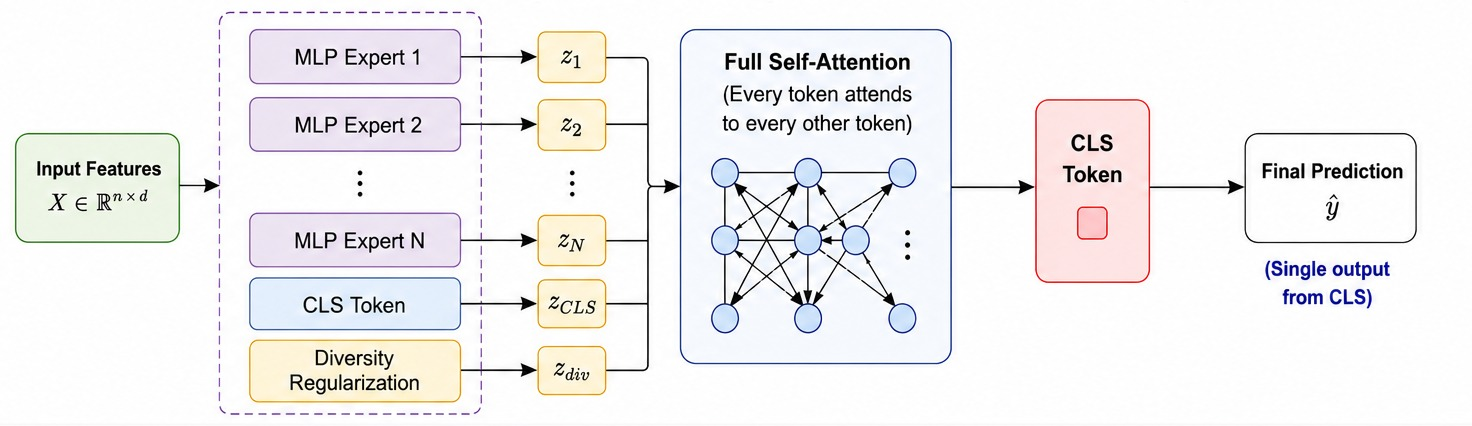
\includegraphics[height=18cm,width=13cm,keepaspectratio]{prev1.jpeg}
    \end{textblock*}
\end{frame}
\begin{frame}{MLPs (V1): Self Attention}
    \begin{itemize}
        \item \textbf{Structure:} An ensemble of $K$ independent MLP ``Experts'' whose outputs are fed into a standard, bi-directional Transformer encoder.
        \item \textbf{Aggregation:} Relies on a global \texttt{[CLS]} token to aggregate spatial information from all experts simultaneously to make a final prediction.
    \end{itemize}
    \vspace{0.3cm}
    \begin{block}{The Bottleneck: Expert Collapse}
        Because attention was symmetric, experts suffered from uniform convergence (learning the exact same feature representations). To counter this, V1 relied heavily on explicit, computationally expensive \textbf{Diversity Regularization}.
    \end{block}

\end{frame}

\begin{frame}{MLPs with Attention (V1): Explicit Diversity Penalties}
    To prevent expert collapse, previous iterations utilized artificial loss penalties:
    \vspace{0.3cm}
    \begin{itemize}
        \item \textbf{Cosine Similarity Penalty:} Pushing expert vectors to be orthogonal.
        \item \textbf{Pearson Correlation Penalty:} Minimizing linear redundancy between expert outputs.
    \end{itemize}
    \vspace{0.3cm}
    \textbf{The Mathematical Flaw:} Optimizing for anti-correlation actively competes with the primary task loss, often forcing experts to learn "opposite" rather than "useful" features. Diversity should be a byproduct of the architecture, not an artificial constraint.
\end{frame}

\section{Related Work}

\begin{frame}{Related Work: Tree-Based Neural Tabular Models}
\begin{columns}[T]

\column{0.48\textwidth}
\begin{block}{Tree-hybrid MLPs (T-MLPs)}
\textbf{Key Idea:} Combines GBDTs and DNNs using sparse tree-guided MLPs.
\begin{itemize}
    \item Structured sparsity and pruning
    \item Mimics tree-like feature interactions
    \item Improves efficiency and generalization
\end{itemize}
\textbf{Relevance:} Supports sparse MLP design inspired by tree learning.
\end{block}

\column{0.48\textwidth}
\begin{block}{TabNet}
\textbf{Key Idea:} Uses sequential attention for interpretable tabular learning.
\begin{itemize}
    \item Sparse attentive feature masks
    \item Step-wise decision reasoning
    \item Visual feature importance
\end{itemize}
\textbf{Relevance:} Shows attention can improve feature selection.
\end{block}

\end{columns}
\end{frame}



\begin{frame}{Related Work: Differentiable Trees and Distillation}
\begin{columns}[T]

\column{0.48\textwidth}
\begin{block}{NODE}
\textbf{Key Idea:} Neural Oblivious Decision Ensembles use differentiable trees.
\begin{itemize}
    \item End-to-end neural training
    \item Shared split functions
    \item Strong tabular performance
\end{itemize}
\textbf{Relevance:} Provides neural approximation of decision trees.
\end{block}

\column{0.48\textwidth}
\begin{block}{DeepGBM}
\textbf{Key Idea:} Distills GBDT knowledge into deep neural networks.
\begin{itemize}
    \item Uses GBDT-learned representations
    \item Compact DNN architecture
    \item Efficient online prediction
\end{itemize}
\textbf{Relevance:} Combines tree-based features with DNN modeling.
\end{block}

\end{columns}
\end{frame}



% ---------------------------------------------------
% PROPOSED ARCHITECTURE
% ---------------------------------------------------
\section{Proposed Architecture: MLPs with Attention (V2)}
\begin{frame}{MLPs with Attention (V2): Sequential Refinement}
    \begin{textblock*}{20cm}(0.8cm,-1.2cm) % Adjust these coordinates if the logo needs to move
        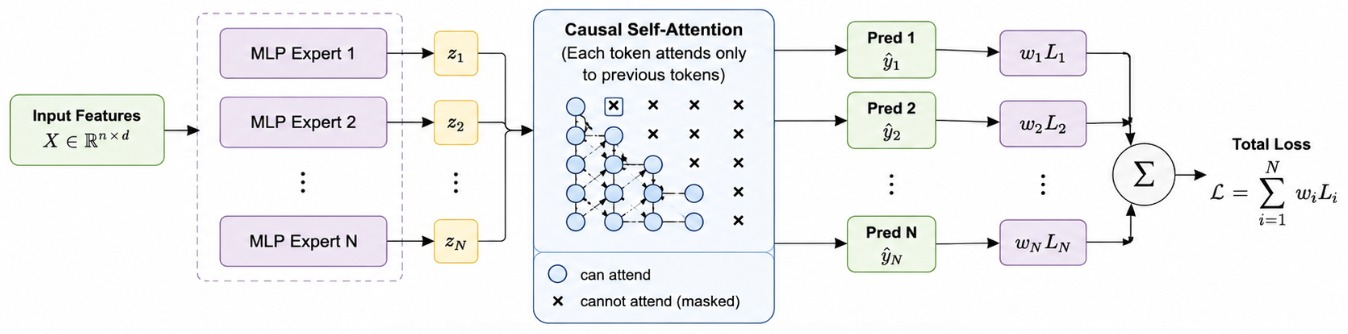
\includegraphics[height=18cm,width=13cm,keepaspectratio]{ours.jpeg}
    \end{textblock*}
\end{frame}
\begin{frame}{From Parallel to Sequential Refinement}
    \begin{block}{The Core Philosophy (V2)}
        We replace symmetric collaboration with \textbf{Sequential Refinement}. By enforcing a strict information hierarchy, we eliminate the need for explicit diversity penalties.
    \end{block}
    \vspace{0.4cm}
    \begin{columns}
        \column{0.5\textwidth}
        \centering \textbf{V1} \\ 
        Parallel / Symmetric \\ 
        Full Attention \\ 
        Artificial Diversity Penalties \\
        Single \texttt{[CLS]} Token Output
        
        \column{0.5\textwidth}
        \centering \textbf{V2 (Our Approach)} \\ 
        Sequential / Residual \\ 
        Causal Masked Attention \\ 
        Architectural (Implicit) Diversity \\
        Dense Step-wise Predictions
    \end{columns}
\end{frame}

\begin{frame}{Key Innovation 1: Causal Attention \& Residuals}
    \textbf{Causal Masking:} A lower-triangular attention mask $M$ ensures that learner $i$ can only attend to features from learners $1 \dots i$. 
    \begin{equation*}
        \text{Attention}(Q, K, V) = \text{softmax}\left(\frac{QK^T}{\sqrt{d_k}} + M\right)V \quad \text{where } M_{ij} = \begin{cases} 0 & \text{if } j \le i \\ -\infty & \text{if } j > i \end{cases}
    \end{equation*}
    
    \textbf{Residual Flow:} Each Transformer block stabilizes gradient flow and preserves base features via Layer Normalization and skip connections:
    \begin{equation*}
        h^{(l+1)} = \text{LayerNorm}\left(h^{(l)} + \text{CausalAttention}(h^{(l)})\right)
    \end{equation*}
\end{frame}

\begin{frame}{Key Innovation 2: Deep Supervision}
    \textbf{Removal of \texttt{[CLS]} Token:} Every token position $i \in \{1 \dots K\}$ produces its own prediction $\hat{y}_i$. We calculate the loss across the entire sequence.
    \vspace{0.3cm}
    \begin{block}{Exponential Loss Weighting}
        \begin{equation*}
            \mathcal{L}_{task} = \sum_{i=1}^K w_i \cdot \text{MSE}(\hat{y}_i, y) \quad \text{where } w_i = \frac{2^i}{\sum_{j=1}^K 2^j}
        \end{equation*}
    \end{block}
    \textbf{Mechanism:} Early predictions (blind to wider context) receive exponentially small weights, acting as gentle feature extractors. The final prediction receives the vast majority of the gradient update.
\end{frame}

% ---------------------------------------------------
% METHODOLOGY
% ---------------------------------------------------
\section{Methodology \& Data Preprocessing}
\begin{frame}{Methodology: Weighted Deep Supervision}
    \begin{columns}
        \column{0.55\textwidth} % Left column for text
        \begin{itemize}
            \item \textbf{Uniform Weighting:} Distributes the loss penalty equally across all steps.
            \item \textbf{Linear Increasing:} Increases the loss penalty in a steady, straight line, ensuring the final prediction is prioritized.
        \end{itemize}
        \vspace{0.1cm}
        \begin{block}{Exponential Weighting}
            \begin{equation*}
                w_i = \frac{2^i}{\sum_{j=1}^K 2^j}
            \end{equation*}
            Perfectly aligns with the "Information Staircase." Early steps receive tiny weights, while the final, fully-informed step drives the primary gradient update.
        \end{block}
        
        \column{0.45\textwidth} % Right column for the image
        \centering
        % Ensure 'weights.png' is uploaded to your Overleaf/LaTeX directory
        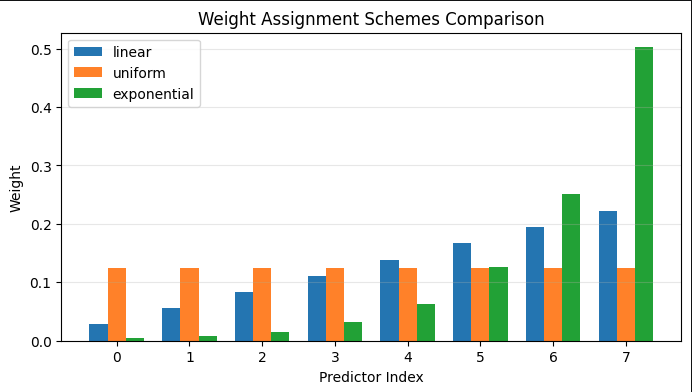
\includegraphics[width=\textwidth, keepaspectratio]{weights.png}
    \end{columns}
\end{frame}
\begin{frame}{Data Preprocessing: RankGauss Transformation}
    \begin{columns}
        \column{0.5\textwidth}
        \textbf{The Limits of StandardScaler}
        \vspace{0.2cm}
        \\
        Standard scaling only shifts the mean and scales variance. Highly skewed tabular data (e.g., housing prices) remains skewed, destabilizing the weak MLPs.
        
        \column{0.5\textwidth}
        \textbf{QuantileTransformer (Normal)}
        \vspace{0.2cm}
        \\
        \begin{itemize}
            \item Re-maps features strictly to a Standard Normal distribution based on empirical ranks.
            \item Aggressively collapses extreme outliers.
            \item \textbf{Impact:} Provides a strictly bounded, smoothed input space, accelerating convergence.
        \end{itemize}
    \end{columns}
\end{frame}

% ---------------------------------------------------
% EXPERIMENTAL RESULTS
% ---------------------------------------------------
\section{Experimental Results}

\begin{frame}{Experimental Setup}
    \begin{table}
        \centering
        \renewcommand{\arraystretch}{1.3} 
        \begin{tabular}{l | l}
            \rowcolor{PrimaryColor} \color{white}\textbf{Parameter} & \color{white}\textbf{Configuration} \\
            Dataset & California Housing (80/20 Split) \\
            \rowcolor{LightGrey} Optimizer & AdamW ($lr=1e-3, \text{weight\_decay}=1e-4$) \\
            Learners ($K$) & 24 \\
            \rowcolor{LightGrey} Embedding Dim. & 32 \\
            Attention Depth & 2 Causal Transformer Blocks \\
            \rowcolor{LightGrey} Head Architecture & Sequential (Linear $\rightarrow$ SiLU $\rightarrow$ Linear) \\
        \end{tabular}
    \end{table}
\end{frame}

\begin{frame}{Results \& Key Findings}
    \begin{itemize}
        \setlength\itemsep{1em}
        \item \textbf{Overall Performance:} Achieved a final validation $R^2$ of \textbf{$\sim$0.812}, significantly outperforming standard MLPs ($\sim$0.72) and bridging the gap to tree-based ensembles.
        \item \textbf{Impact of Exponential Weighting:} Outperformed inverse and linear weighting schemes. By not severely punishing early weak learners, gradient thrashing was eliminated.
        \item \textbf{Ablation Insight:} The integration of \textit{Residual Connections} and \textit{LayerNorm} proved to be absolute prerequisites for successfully training deeper transformer blocks without vanishing gradients.
    \end{itemize}
\end{frame}

% ---------------------------------------------------
% CONCLUSION
% ---------------------------------------------------
\section{Conclusion}

\begin{frame}{Conclusion \& Future Work}
    \textbf{Conclusion:} 
    \begin{itemize}
        \item The proposed architecture successfully translates the sequential refinement of GBDTs into a purely neural, differentiable framework.
        \item Causal masking intrinsically solves the expert collapse problem without artificial diversity constraints.
    \end{itemize}
    \vspace{0.4cm}
    \textbf{Future Work:}
    \begin{itemize}
        \item Exploring sparse attention mechanisms for larger $K$ values.
        \item Benchmarking it against complex categorical datasets.
        \item Investigating dynamic weighting mechanisms (e.g., Learnable Deep Supervision Weights).
    \end{itemize}
\end{frame}

\begin{frame}{References}
    \footnotesize
    \begin{enumerate}
        \item Previous Work (MLPs with Attention (V1) Internal Report): Differentiable Neural Architectures for Tabular Data.
        \item Chen, T., \& Guestrin, C. (2016). XGBoost: A Scalable Tree Boosting System. \textit{KDD}.
        \item Vaswani, A., et al. (2017). Attention Is All You Need. \textit{NeurIPS}.
        \item Lee, C. Y., et al. (2015). Deeply-Supervised Nets. \textit{AISTATS}.
        \item Scikit-Learn Developers. \textit{QuantileTransformer Documentation}.
    \end{enumerate}
\end{frame}

% --- Q&A SLIDE ---
\begin{frame}[plain]
    \vfill
    \begin{center}
        \vspace{0.8cm}
        \textcolor{PrimaryColor}{\Huge \textbf{Thank You}} \\
        \vspace{0.8cm}
        \large \textbf{Questions \& Discussion} \\
        \vspace{0.5cm}
        % \normalsize 
        % \textit{Email:} [Your Email] \\
        % \textit{GitHub:} [Your Repo Link]
    \end{center}
    \vfill
\end{frame}

\end{document}